\documentclass{beamer}
\mode<presentation>
{\usetheme{default}
 \usecolortheme{default}
 \usefonttheme{default}
 \setbeamertemplate{navigation symbols}{}
 \setbeamertemplate{caption}[numbered]} 
\usepackage[english]{babel}
\usepackage[utf8x]{inputenc}
\usepackage{graphicx}
\usepackage[alf]{abntex2cite}
\usepackage{amsmath}

\usepackage{multibib}
\usepackage{mathrsfs,amsmath}
\usepackage{longtable}
\usepackage{amssymb}
\usepackage{url}
\usepackage{pgfpages}
\usepackage{enumerate}
\usepackage{color}
\usepackage{ifthen}
\usepackage{capt-of}


%%%%%%%%%%%%%%%%%%%%%%%%%%%%%%%%%%%%%%%%%%%%%%
\title[Qualify presentation]{High Performance Computing applied to\\ Spectral Simulation}
\author{Péricles Lopes Machado}
\institute{PROGRAMA DE PÓS-GRADUAÇÃO EM ENGENHARIA DE MINAS, METALÚRGICA E DE MATERIAIS\\ Universidade Federal do Rio Grande do Sul}
\date{17th April 2017}
%%%%%%%%%%%%%%%%%%%%%%%%%%%%%%%%%%%%%%%%%%%%%%

\begin{document}

%%%%%%%%%%%%%%%%%%%%%%%%%%%%%%%%%%%%%%%%%%%%%%
\begin{frame}
  \titlepage
\end{frame}
%%%%%%%%%%%%%%%%%%%%%%%%%%%%%%%%%%%%%%%%%%%%%%

%%%%%%%%%%%%%%%%%%%%%%%%%%%%%%%%%%%%%%%%%%%%%%
\section[]{}
\begin{frame}{Table of contents}
	\tableofcontents
\end{frame}
%%%%%%%%%%%%%%%%%%%%%%%%%%%%%%%%%%%%%%%%%%%%%%

%%%%%%%%%%%%%%%%%%%%%%%%%%%%%%%%%%%%%%%%%%%%%%%%%%%
% introducao
\section{Motivation}

\begin{frame}{Motivation}
  \begin{itemize}
    \item Geostatistical Simulation is an important tool to model the uncertainty in geo-referenced datasets.
    \item A set of realizations is generated to approximate the uncertainty space.
    \item Simulation is an expensive computational task.
    \item There are two main methodologies to generate the realizations: Sequential Simulation and Spectral Simulation.
     \item The Sequential Simulation is the most used Geostatistical Simulation algorithm.
  \end{itemize}
\vskip 1cm
\end{frame}

\subsection{Problem 1: How to reduce the execution time of Geostatistical Simulations?}
\begin{frame}{Problem 1}	
How to reduce the execution time of Geostatistical Simulations? 
\end{frame}

\begin{frame}{How to reduce the execution time of Geostatistical Simulations?}
	\begin{itemize}
      \item The execution time of an algorithm can be reduced using two main strategies: parallelization of the fundamental logic blocks and/or changing the key ideas used to implement the algorithm.
		\item In computer science, the High Performance Computing (HPC) is a set of  Hardware and Software methodologies to reduce the execution time of complex computational tasks.    
    \end{itemize}
\end{frame}

\begin{frame}{How to reduce the execution time of Geostatistical Simulations?}
	\begin{itemize}
    	\item The algorithm parallelization isn't a general solution, because is needed to study the nature of the problem to identify what tasks can be executed simultaneously.
        \item Task interdependence is the main problem faced during the algorithm parallelization.
        \item  The synchronization of tasks being executed in parallel reduces the efficiency of the parallelization.
    \end{itemize}
\end{frame}

\begin{frame}{How to reduce the execution time of Geostatistical Simulations?}
	\begin{itemize}
    	\item Lets discuss the Problem 1.
        \item What is the best strategy to reduce the execution time of Geostatistical Simulations:
        \begin{itemize}
        	\item Parallelize the Sequential Simulation;
        	\item Use other algorithm;
        	\item Or, parallelize other algorithm?
        \end{itemize}
    \end{itemize}
\end{frame}

\subsection{Why parallelize the Sequential Simulation isn't the best solution?}
\begin{frame}{Why parallelize the Sequential Simulation isn't the best solution?}
	\begin{itemize}
    	\item The Sequential Simulation is dependent of a random path  \cite{goovaerts1997geostatistics}.
        \item The random path is used to define the simulation order of the nodes.
        \item When a node is simulated, it is transformed in conditioning data.
        \item That is the problem: Sometimes two or more close nodes to be simulated are sharing the neighborhood. In other words, these two or more nodes are conditioning data to the others. This is called a \textbf{Conflict Zone} (Fig. \ref{conflict_zone}).
    \end{itemize}
\end{frame}

\begin{frame}{Why parallelize the Sequential Simulation isn't the best solution?}
\begin{figure}[h]
  \caption{Conflict zone between two neighborhoods. The red stars are two points to be simulated in a given moment.}
  \centering
    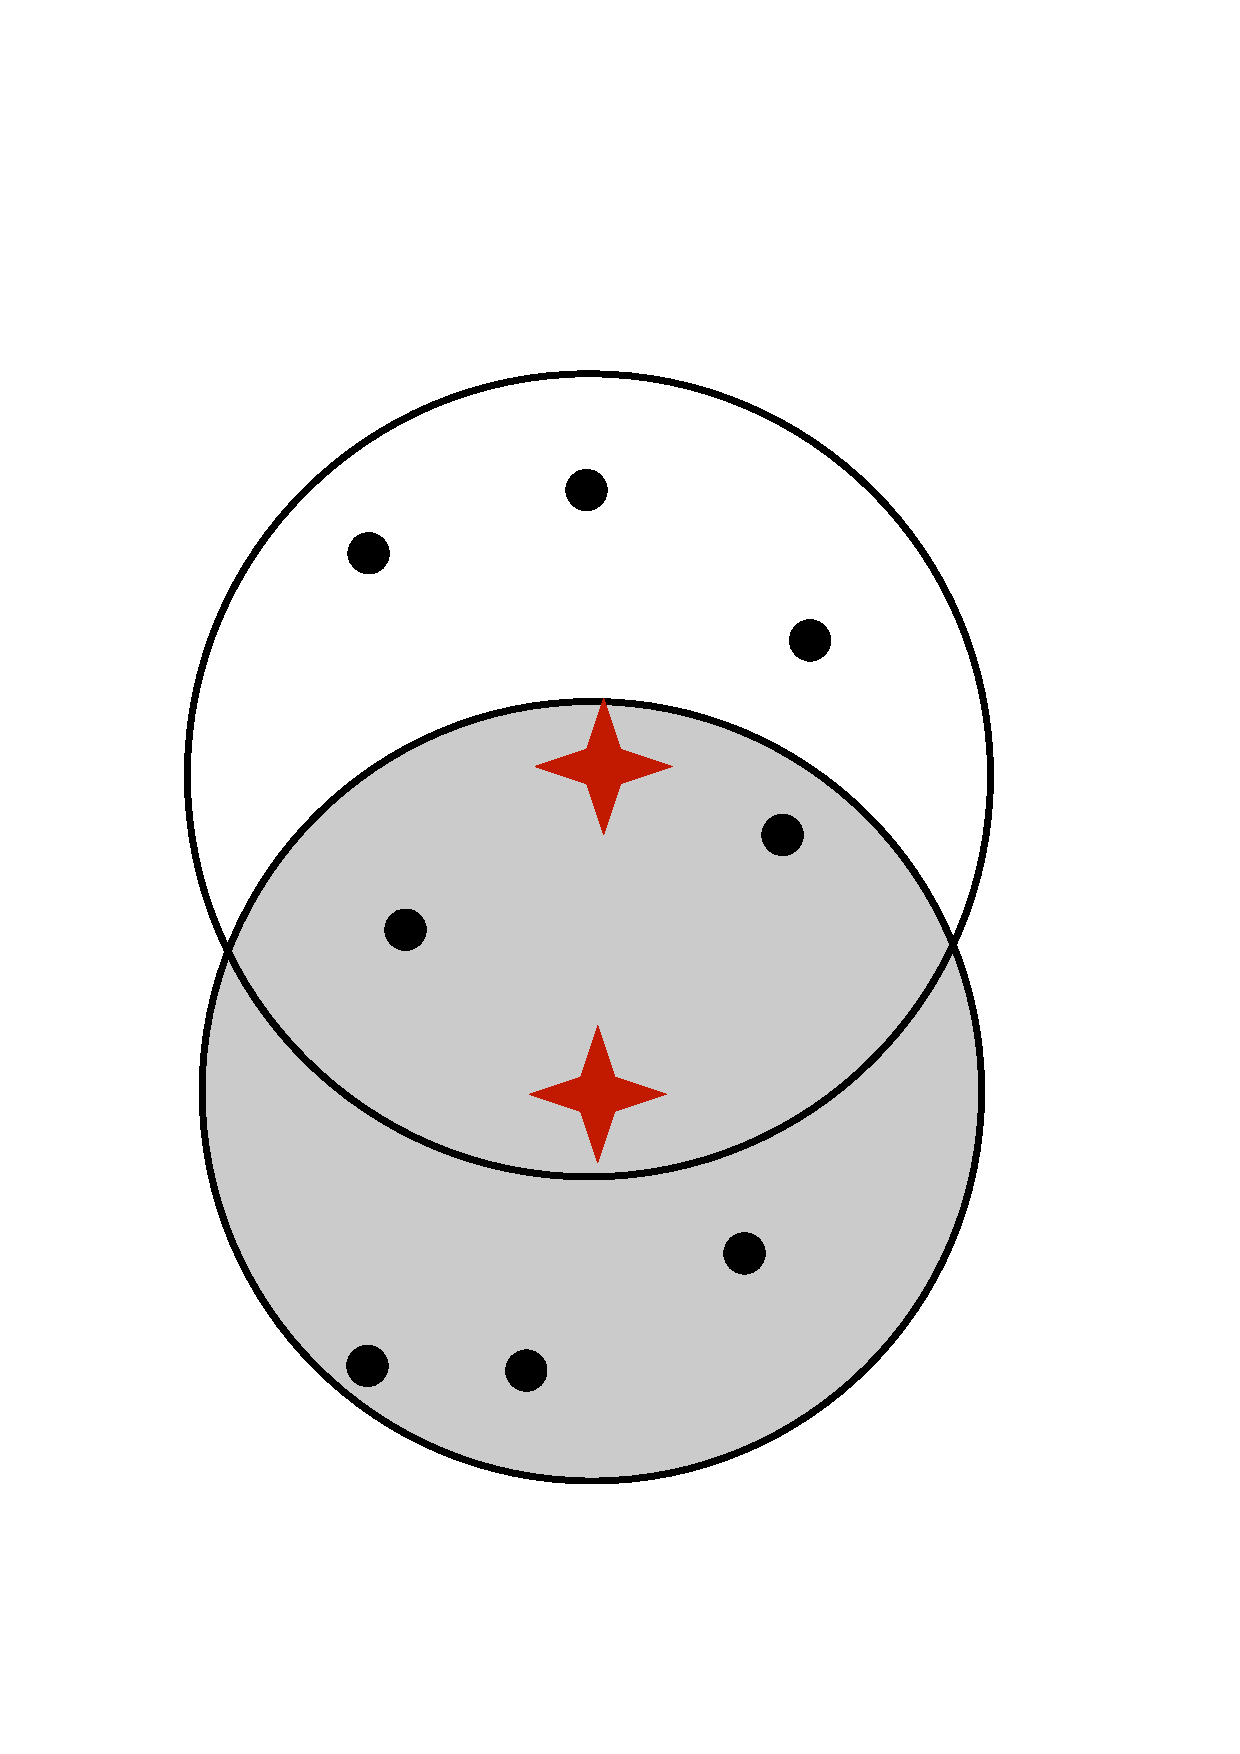
\includegraphics[width=0.4\textwidth,angle=90]{figs/conflict_zone.pdf}
    \label{conflict_zone}
\end{figure}

\end{frame}

\begin{frame}{Why parallelize the Sequential Simulation isn't the best solution?}
	\begin{itemize}
    	\item In literature, there are five ways to lead with the conflict zones \cite{mariethoz2010general}:
        \begin{enumerate}
        	\item Parallelize the krigings executed during each node simulation. \cite{nunes2010parallelization}
            \item Analyze the random path to identify the nodes in non-conflicting neighborhoods and simulate them in parallel. \cite{vargas2007parallelization}
            \item Use Message Passage to synchronize the execution and check if a sub-set of nodes in the random path can be simulated in parallel. \cite{mariethoz2010general}
            \item Divide the grid in independent fields and generate the random paths for each independent field. This strategy is highly dependent of the spatial continuity. \cite{rasera2015conflict}
            \item The trivial solution: execute in parallel the simulation of several realizations (each realization is executed using the original sequential algorithm).
        \end{enumerate}
    \end{itemize}
\end{frame}

\begin{frame}{Why parallelize the Sequential Simulation isn't the best solution?}
	\begin{itemize}
    	\item The trivial solution is memory expensive and useless during the calibration of the model parameters. Also, running in parallel several simulations of large grids demands a lot of memory, what reduces significantly the parallelization performance.
        \item Divide the grid in independent fields is a good solution when the data has a low spatial continuity in a direction. But, this is a limitation to the number of fields that can be simulated in parallel.
        \item Synchronize the execution steps demands the creation of a non-trivial execution manager to define the nodes or the kriging systems to be used in a given moment.
    \end{itemize}
\end{frame}


\begin{frame}{Why parallelize the Sequential Simulation isn't the best solution?}
	\begin{itemize}
    	\item The synchronization of execution steps and the strategy to divide the grid in independent fields allows the parallelization in the path level. This is useful during the parameter calibration.
        \item These are the main approaches to parallelize the Sequential Simulation. With exception of the trivial solution all solutions generate more complex version of the simulation algorithm and have limitations due the nature of the random path or the spatial continuity. These limitations impact directly on the efficiency of the parallelization.
    \end{itemize}
\end{frame}

\subsection{Problem 2: If parallelize the Sequential Simulation isn't the best solution, what to do?}
\begin{frame}{Problem 2}	
If parallelize the Sequential Simulation isn't the best solution, what to do? 
\end{frame}

\begin{frame}{If parallelize the Sequential Simulation isn't the best solution, what to do?}
	\begin {itemize}
		\item Parallelize the kriging is trivial, because to estimate each grid node it's needed only the conditioning data. Also, the conditioning data is immutable during the estimation. This allows the parallel execution of the node estimations. In computer science this type of algorithms is called \textit{embarrassingly parallel} \cite{wilkinson1999parallel}.
    
    	\item This raises a question: ``Are there some way to develop a parallel simulation algorithm \textit{embarrassingly parallel}?''
    \end {itemize}
\end{frame}

\begin{frame}{If parallelize the Sequential Simulation isn't the best solution, what to do?}
	\begin {itemize}
		\item An \textit{embarrassingly parallel} algorithm allows the developer to use all possible parallelization strategies and technologies. And, in theory, the parallelization in this case is ``perfect'', allowing to achieve the maximum speed-up in all problem instances. 
        \item Due the random path, the Sequential Simulation is \textit{embarrassingly parallel} only in the realization level, what is a big limitation when a large grid is simulated.
        \item High memory consumption reduces significantly the execution performance because the CPU cache is overloaded. The  good use of CPU cache is a key to high performance.
    \end {itemize}
\end{frame}


\begin{frame}{If parallelize the Sequential Simulation isn't the best solution, what to do?}
	\begin {itemize}
    	\item Reduce the memory consumption is an important way to improve the execution performance.
        \item Other bottleneck during the parallelization is the synchronization. Synchronization creates a sequential stage in the parallel algorithm. In other words, during the synchronization it isn't possible to use the other available CPUs.
        \item The main parallelization strategies to the Sequential Simulations are based on the nature of the spatial continuity (high continuity is a limitation to the parallelization scalability), synchronization (a sequential step is added to organize the parallel execution of nodes) or high memory consumption (the realizations are simulated in parallel in different CPUs).
    	
    \end {itemize}
\end{frame}


\begin{frame}{If parallelize the Sequential Simulation isn't the best solution, what to do?}
	\begin{itemize}
    	\item This raises a question: ``Are there some way to develop an  \textit{embarrassingly parallel} and memory efficient simulation algorithm?''
        \item The answer is: ``YES''.
        \item The spectral simulation is the way to achieve an \textit{embarrassingly parallel} and memory efficient simulation algorithm. 
    \end{itemize}
\end{frame}


\section {Thesis statement}
\begin{frame}{Thesis statement}
The previous discussion presented the motivation to the thesis statement:


\begin{block}{}
``High performance computing applied to spectral simulation is the best approach to develop parallel simulation algorithms.''
\end{block}

\end{frame}

\section{Goals}
\begin{frame}{Goals}

The main goal of this is to investigate the possibility of building a new generation of geostatistical software that uses efficiently the resources of a modern computational infrastructure (like GPUs, clusters, multi-core processors and HPC libraries).

To accomplish the thesis goal the following geostatistical algorithms will be explored:

\begin{itemize}
	\item Spectral simulation: Fourier Integral Method (FIM) and Turning Bands (TBSIM).
    \item Covariance table generation;
\end{itemize}
\end{frame}


\section{Methodology}
\begin{frame}{Methodology}
	\begin{itemize}
		\item The \textit{SGeMS} \cite{remy2009applied} will be used as software platform to the algorithm development, once it has many fundamental building blocks for geostatistical algorithms.
        \item A distributed version of the Fourier Integral Method will be developed and applied in practical situations. The algorithm limitations and challenges will be explored.
        \item Methodologies to generate automatically or semi-automatically covariance table will be investigated.
	\end{itemize}
\end{frame}

\section{Contributions}
\begin{frame}{Contributions}
	\begin{itemize}
        \item New methodologies to generate automatically or semi-automatically covariance table and density spectrum.
    	\item New parallelization strategies to implement distributed version of spectral simulation algorithms using efficiently the resources available in a modern computational infrastructure.
        \item New architectures and methodologies to develop modern geostatistical software. 
    \end{itemize}
\end{frame}

\section{Outcomes}
\begin{frame}{Outcomes}
	At the end of this work, it will delivered:
    \begin{itemize}
        \item A new version of \textit{SGeMS}, called \textit{Ar2GeMS HPC} to provide distributed version of geostatistical algorithms (Kriging, SGSIM, TBSIM, and so on). This software will simplify the creation of plugins that need to use a set of different computers to execute a complex task.
    	\item A new package of HPC implementations of a variety of fundamental geostatistical algorithms;
        \item An API and a distributed computational infrastructure to execute geostatistical workflows on a very large dataset;
        \item A new software tool to simplify the development of HPC geostatistical algorithms. 
    \end{itemize}
\end{frame}





\section{Covariance table generation}
\begin{frame}{Covariance table generation}
The covariance table $C$ is a data structure used to model the covariances on a grid. Each entry $C(hx,hy,hz)$ gives the covariance between points $p_1 = (x_1, y_1, z_1)$ and $p_2 = (x_2, y_2, z_2)$ apart of $(hx, hy, hz)$, where $hx = x_2 - x_1$, $hy = y_2 - y_1$ and $hz = z_2 - z_1$.

There are two main ways to generate this table:
\begin{itemize}
	\item Implicit modeling: The data is used directly to generate the table. A smoothing strategy is needed to eliminate numeric artifacts and generate a positive-definite model\cite{cov.paper}.
    \item Explicit modeling: This is the traditional approach. An explicit model using admissible functions is used to fit a curve in an experimental variogram generated from data. From this model the covariance table can be built for every lag at any direction.
\end{itemize}
\end{frame}

\begin{frame}{The relationship between Covariance Table and Density Spectrum}
The density spectrum $s(\omega)$ is the Fourier Transform of the covariance table. As the covariance table is an even function, i. e., $C(h=(hx,hy,hz))=C(-h=(-hx,-hy,-hz))$, then the density spectrum is real and even.

$$
s(\omega)=\mathscr{F}\left[ C(h) \right]
$$
\end{frame}

\begin{frame}{The Bochner's Theorem}
An important result of the Theory of Fourier Transform is the Bochner's Theorem \cite{bochner1939additive}:

\begin{block}{}
A function $f(y)$ is positive-definite if it is the Fourier Transform of a real function $g(y) \geq 0$.
\end{block}
\end{frame}

\begin{frame}{Generating covariance tables using the Bochner's Theorem}
The Bochner's Theorem is an important tool to generate admissible covariance table $C(h)$ from data, as the density spectrum of a covariance table is a real function $s(\omega) \geq 0$.

Before generating the admissible covariance table $C(h)$ is needed to build an experimental covariance table from data. This task can be done using the Marcotte approach \cite{fast.var.paper}, where Fast Fourier Transform (FFT) \cite{johnson2008implementing} is used to fast generate of an experimental covariance table. Or, the experimental covariance table can be generated using a geometric algorithm based on angular and bandwidth tolerances. 
\end{frame}


\begin{frame}{Generating covariance tables using the Bochner's Theorem}

\begin{itemize}
\item After generating the experimental covariance table $\tilde{C}(h)$,  some information may be missing at some lags $h$ or there are many artifacts. In this case, it is needed to fill the missing data and remove the artifacts. An interpolation and smoothing algorithm is needed to adjust the experimental model $\tilde{C}(h)$ and generate an admissible covariance table $C(h)$. 

\item Yao \cite{cov.paper} presents an algorithm to execute the model interpolation and spectrum smoothing.
\end{itemize}

\end{frame}


\begin{frame}{The Yao's algorithm}

\begin{enumerate}
\item Let $\tilde{C}(h)$ be an interpolated experimental covariance model generated using the data with a radial inverse distance interpolation, for example. This will be the first step to smooth the covariance model and remove artifacts. However, it is not assured that model is positive-definite.
\item $\tilde{C}(h)$ is even and real. Then the Bochner's Theorem can be used.
\item Let $\tilde{s}(\omega)$ be the density spectrum of $\tilde{C}(h)$. To generate a positive-definite function $C(h)$ is enough to smooth $\tilde{s}(\omega)$ using a moving average in each point of the density spectrum $\tilde{s}(\omega)$. 
\item Let $s(\omega)$ be the smoothed density spectrum generated in the previous step. Applying the Inverse Fourier Transform $\mathscr{F}^{-1}$ in $s$, an admissible covariance table $C(h) = \mathscr{F}^{-1}[s(\omega)]$ is generated.
\end{enumerate}

\end{frame}

\begin{frame}{A covariance table figure}
A smoothed covariance table generated using the Walker Lake data-set and Yao's algorithm.
\begin{figure}[!ht]
  %\caption{A smoothed covariance table generated using the Walker Lake data-set and Yao's algorithm.}
  \centering
    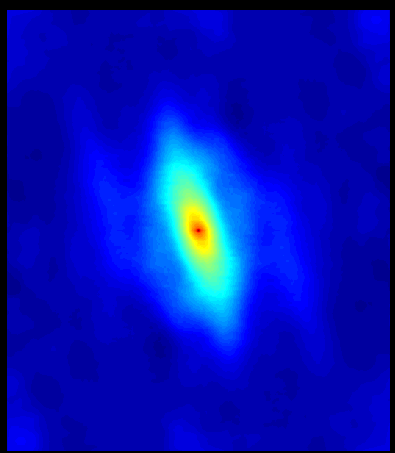
\includegraphics[height=0.4\textheight, width=0.6\textwidth]{figs/cov_table_fig.png}
    \label{cov_table_ex.fig}
\end{figure}

\end{frame}

\begin{frame}{A density spectrum figure}
A smoothed density spectrum generated using the Walker Lake data-set and the Yao's algorithm.
\begin{figure}[!ht]
  %\caption{A smoothed density spectrum generated using the Walker Lake data-set and the Yao's algorithm.}
  \centering
    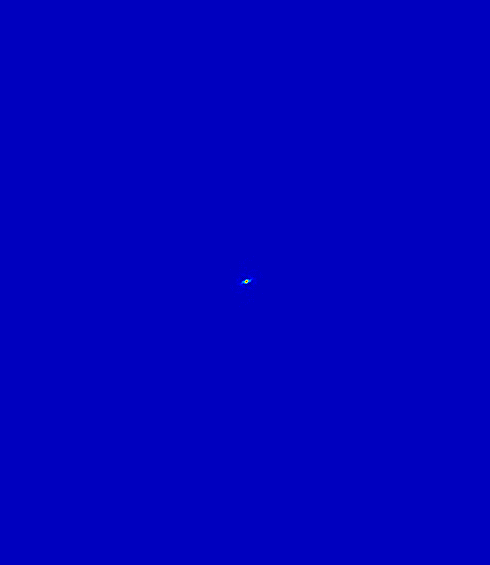
\includegraphics[height=0.5\textheight]{figs/dens_spec.png}
    \label{dens_spec.fig}
\end{figure}
\end{frame}


\begin{frame}{Why covariance tables are useful?}
\begin{itemize}
\item The covariance table $C(h)$  can be used in traditional simulation/estimation algorithms as Sequential Gaussian Simulation, Kriging, etc.
\item It can be used in the conditioning step of spectral simulations such as Turning Bands and Fourier Integral Method.
\item The covariance modeling is the most time consuming stage of most geostatistical workflows. A semi-automatic covariance table modeling tool could reduce this time. Mainly, when a multi-variate model based on MLC  is being built \cite{cov.paper}.
\end{itemize}
\end{frame}

\begin{frame}{The covariance table modeling challenges}

\begin{itemize}
\item Yao's algorithm is powerful. But, it is highly dependent of the quality of input data. It demands a good sampling of simulation/estimation domain.

\item To deal with this limitation an explicit model is needed or an auxiliary  model containing the expected covariance would be required.

\item How this auxiliary model can be generated? Derived from a trend map obtained by Radial Base Function or some machine learning estimation technique?

\item This is an open question to be answered.
\end{itemize}

\end{frame}



\section{Fourier Integral Method}
\begin{frame}{Fourier Integral Method}
  \begin{itemize}
  	\item The density spectrum $s(\omega)$ created in the last sections can be used directly to generate unconditional realizations. This is the \textit{Fourier Integral Method (FIM)} \cite{pardo1993fourier}.
    \item The covariance table $C(h)$ can be generated using the following equation:
    $$
    C(h) = z * z = \mathscr{F}^{-1}[Z(\omega) \cdot Z(\omega)],
    $$
    
    $$
    s(\omega) = Z(\omega) \cdot Z(\omega),
    $$
    where $z(p)$ is data function in the point $p=(x,y,z)$, $*$ is the convolution operation and $Z(\omega) = \mathscr{F}[z(p)]$,
    \item Remembering that $Z(\omega)$ can be written as $Z(\omega)=|Z(\omega)|e^{i\theta}$. And if a function $f(y)$ is real, the angle $\theta$ is 0 for all $y$. 
    \item Then, the density spectrum $s(\omega)$ is given by $s(\omega) = |Z(\omega)|^2$.
  \end{itemize}
\end{frame}

\begin{frame}{Fourier Integral Method}
  \begin{itemize}
  	\item The density spectrum $s(\omega)$ can be used  to recover the magnitude of the original data function $z(p)$, because $|Z(\omega)| = \sqrt{s(\omega)}$. Remembering that $s(\omega) \geq 0$ is a positive function. Also, $\sum |s(\omega)| = C(0)$.
    \item In the FIM simulation, the lost angle $\theta(\omega)$ is re-added to the density spectrum  $\sqrt{s(\omega)}$. And data conditioning is realized using error kriging.
    \item The unconditional simulation is done generating random angles $\theta(\omega)$ from an uniform distribution $U(-\pi,\pi)$.
    \item Then, the unconditional realization $z^{r}(p)$ is generated using the equation $z^{r}(p) = \mathscr{F}^{-1}[\sqrt{s(\omega)}e^{i\theta(\omega)}]$. Without loss of generality, let assume that $Z^{r}(p)=\sqrt{s(\omega)}e^{i\theta(\omega)}$ is even (this assure that the inverse is a real function).
  \end{itemize}
\end{frame}

\begin{frame}{Unconditional simulation using Covariance table and FIM}
\begin{figure}[!ht]
  \caption{Example of unconditional simulation using a smoothed covariance table generated using the Walker Lake dataset.}
  \centering
    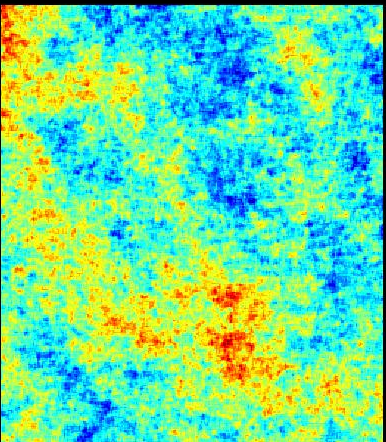
\includegraphics[height=0.5\textheight]{figs/sim_cov_table.png}
    \label{cov_table_sim.fig}
\end{figure}
\end{frame}


\begin{frame}{Advantages of Fourier Integral Method}
\begin{itemize}
	\item FIM doesn't need a random path.
    \item The generated covariance table from data can be used directly to generate the unconditional simulations and conditioning.
    \item FIM is embarrassingly parallel.
\end{itemize}
\end{frame}

\begin{frame}{Drawbacks of Fourier Integral Method}
\begin{itemize}
	\item It's highly dependent on the correct adjust of the simulation grid. The grid discretization (cell size) is directly related to the quality of simulation. A more continuous spatial input data demands a small cell size. This fact is explained by the Nyquist Sampling Theorem \cite{pardo1993fourier}. 
    \item The FFT in non-equally sampled vector of data isn't a trivial problem \cite{keiner2009using}.
\end{itemize}
\end{frame}





\section{Turning Bands}

\begin{frame}{Turning Bands}
  \begin{itemize}
  	 \item The Turning Bands algorithm has been designed by Matheron \cite{matheron1973intrinsic}.
    \item Turning Bands is an algorithm to transform the simulation of a Gaussian random function with covariance $C$ in $M$ simulations of independent stochastic processes with covariances $C_\theta$ (where $\theta$ is a direction and $C_\theta$ is called \textit{Spectral representation of the covariance $C$}).
    \item To generate the simulations, $M$ lines are created in different directions in a standard unit sphere in $\mathbb{R}^d$, 1D independent simulations are computed in each direction and the results are combined to generate the simulation in $\mathbb{R}^d$. 
    \item This methodology is similar to the Fourier Integral Method, where the simulation in $\mathbb{R}^d$ is transformed in the independent simulation of the angles $\theta(\omega)$ (phase simulation).
  \end{itemize}

\end{frame}

\begin{frame}{Turning Bands}
\begin{itemize}
\item Each covariance type is simulated using a specific algorithm. \cite{emery2006tbsim}
\item To simulate covariances that are result of a linear combination of basic models (spherical, exponential, Gaussian, nugget, etc...), we simulate independently each model and the results are combined.
\item Because the 1D simulation in each node is completely independent, 
we can easily parallelize the simulation in space without any synchronization technique. 
\item The Turning Bands method can be seen as a generalization of the spectral method \cite{lantuejoul2013geostatistical}. Remembering, that we can use FIM 1D to simulate the 1D covariance models. 
\end{itemize}
\end{frame}

\begin{frame}{Turning Bands}
\begin{itemize}
 \item The relationship between the simulation of independent stochastic processes and the simulation of the original Gaussian random function is given by 
 \begin{equation}
  Y^{(n)}(x) = \frac{1}{\sqrt{n}} \sum_{k=1}^{n} X_k(<x,\theta_k>), x \in \mathbb{R}^d
 \end{equation}
 where $(\theta_n, n \in \mathbb{N})$ is a sequence of directions in an unit sphere $S_d$ and $(X_n, n \in \mathbb{N})$ is a sequence of
 independent stochastic processes with covariance $C_{\theta_n}$. $\rho_n = <x, \theta_n>$ is the projection of the vector
 $x$ in direction $\theta_n$ and $X_n(\rho_n)$ is the spectral representation of the Gaussian random function $Y^{(n)}(x)$ in
 the direction $\theta_n$.
\end{itemize}
\end{frame}

\begin{frame}{Turning Bands}
\begin{itemize}
\item The covariance $C^{(n)}(h)$ of $Y^{(n)}(x)$ is described by
\begin{equation}
C^{(n)}(h) = \frac{1}{n} \sum_{k=1}^{n} C_{\theta_k}(<h, \theta_k>)
\end{equation}

where $C_{\theta_n}(<h, \theta_n>)$ is the spectral representation of the covariance $C^{(n)}(h)$.

\item If the covariance $C$ is isotropic, i.e., can be written as $C(h)=C_d(|h|)$ for some scalar function $C_d$ defined on 
$\mathbb{R}^{+}$, then the relationship between $C_1$ and $C_d$ is given by

\begin{equation}\label{eq_cov_d}
 C_d(r) = 2 \frac{(d-1)\omega_{d-1}}{d\omega_{d}} \int_{0}^{1}(1-t^2)^(\frac{d-3}{2})C_1(tr) dt
\end{equation}

where $\omega_{d}$ stands, as usual, the d-volume of the unit ball in $\mathbb{R}^d$. 
\end{itemize}
\end{frame}


\begin{frame}{Turning Bands}
 \begin{itemize}
  \item If $d=3$, the equation (\ref{eq_cov_d}) is reduced to
  \begin{equation}
    C_3(r) = \int_{0}^{1}C_1(tr)dt
  \end{equation}
  
  or equivalently
  \begin{equation}
   C_1(r) = \frac{d}{dr}rC_3(r)
  \end{equation}

  Curiously, for $d=2$ the relationship is more complicated
  \begin{equation}
   C_2(r) = \frac{1}{\pi}\int_{0}^{\pi}C_1(r sin(\theta))d\theta
  \end{equation}
  
  and
  
  \begin{equation}
   C_1(r) = 1 + r \int_{0}^{\pi/2} \frac{d}{dr}C_2(r sin \theta) d\theta
  \end{equation}


 \end{itemize}

\end{frame}

\begin{frame}{The Turning Bands algorithm} 

 Keeping in mind the previous results, the Turning Bands algorithm can be written as:
 
\begin{block}{}\label{tb.algo}
\begin{enumerate}
 \item Generate a set of directions $\theta_1, ..., \theta_n$ such that $\frac{1}{n}\sum_{k=1}^{n}\delta_{\theta_k} \approx \varpi$.
 \item Generate independent standard stochastic processes $X_1, ..., X_n$ with covariances functions $C_{\theta_1}, ..., C_{\theta_n}$.
 \item Compute $\frac{1}{\sqrt{n}}\sum_{k=1}^{n}X_k(<x, \theta_k>)$ for any $x \in D$.
\end{enumerate}
\end{block} 

In this algorithm, $D$ is the simulation domain, $\delta_{\theta_n}$ is a distribution where $\sum_{k=1}^{n}\delta_{\theta_k}$
converges weakly to $\varpi$, the uniform distribution over $S_d$ (unit sphere in $\mathbb{R}^d$). 
\end{frame}


\begin{frame}{Turning Bands: Generating the directions}
There are three main ways to generate directions $\theta_n$ satisfying the TB condition:
\begin{itemize}
 \item Arrange $\theta_n$ regularly on $S_d$. This approach is efficient in $d=2$, but for dimensions greater than 2
 this solution doesn't work well. In $d=3$, for example, the maximum number of regular directions is equal to 15.
 \item Generate $\theta_n$ using a uniform distribution in $S_d$ works. 
 But, using this method, the convergence of $\frac{1}{n}\sum_{k=1}^{n}\delta_{\theta_k}$
 is very slow, i.e., we need many lines to generate good results.
 \end{itemize}

\end{frame}


\begin{frame}
\frametitle{Turning Bands: Generating the directions}
\begin{itemize}
 \item Use a sequence with weak discrepancy. For $d=3$, \cite{freulon1994conditional} propose the sequence:
 \begin{equation}
 \begin{aligned}
  u_n = \frac{a_0}{2} + \frac{a_1}{4} + ... + \frac{a_p}{2^{p+1}} \\
  v_n = \frac{b_0}{3} + \frac{b_1}{9} + ... + \frac{b_p}{3^{q+1}} \\
  \theta_n = \left( \cos(2\pi u_n) \sqrt{1-v_n^2}, \sin(2\pi u_n) \sqrt{1 - v_n^2}, v_n \right)
  \end{aligned}
 \end{equation}
 
 where $a_i = 0, 1$ and $b_j = 0, 1, 2$ and $n=a_p...a_2a_1a_0=b_q...b_2b_1b_0=a_0 + 2a_1 + ... + 2^pa_p=b_0+3b_1+...3^qb_q$. In other
 words, $a_i$ and $b_j$ are the digits of the binary and ternary representation of $n$, respectively.
\end{itemize}
\end{frame}

\begin{frame}{Turning Bands: Generating the directions}

The Freulon's algorithm produces $\theta_n$ as far as possible from $\theta_1, ... , \theta_{n-1}$ and fills the sphere $S_d$ as
fast as possible. How we can see in the Figs. \ref{fig:freulon_algo_10_bands}, \ref{fig:freulon_algo_100_bands}, 
\ref{fig:freulon_algo_1000_bands}, using 1000 bands is possible to generate a dense set of points filling the sphere $S_d$.

In the practice, the Freulon's algorithm assure a fast convergence to the TB algorithm. Generally, to large datasets, using 1000 or 2000 directions
it is possible to generate good results. To generate other configurations of bands, we can rotate the bands using a random rotation.
\end{frame}


\begin{frame}
\frametitle{Turning Bands: Generating the directions}
\begin{figure}
\begin{center}
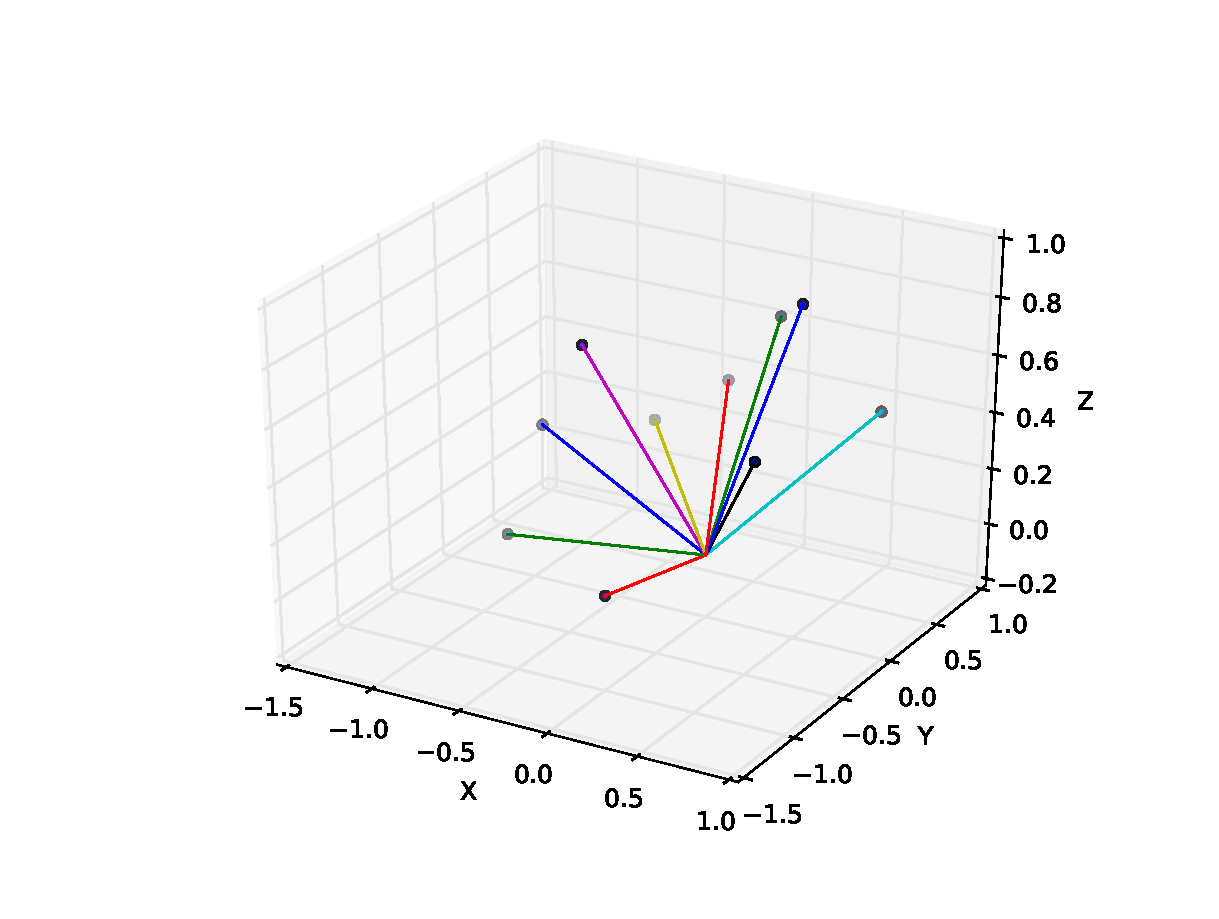
\includegraphics[height=0.7\textheight]{figs/freulon_algo_10_bands.pdf}
\end{center}
\caption{10 bands generated using the Freulon's algorithm}
\label{fig:freulon_algo_10_bands}
\end{figure}
\end{frame}


\begin{frame}
\frametitle{Turning Bands: Generating the directions}
\begin{figure}
\begin{center}
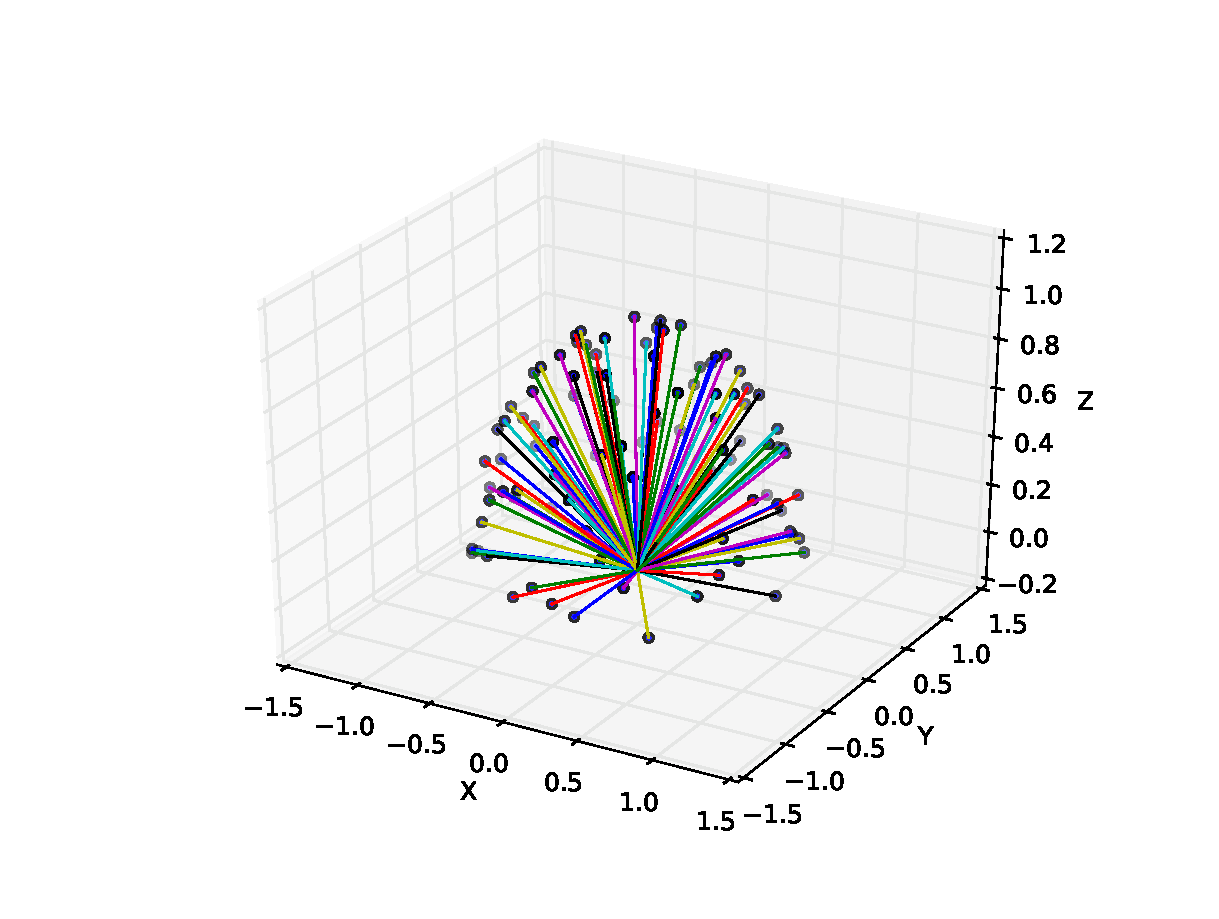
\includegraphics[height=0.7\textheight]{figs/freulon_algo_100_bands.pdf}
\end{center}
\caption{100 bands generated using the Freulon's algorithm}
\label{fig:freulon_algo_100_bands}
\end{figure}
\end{frame}


\begin{frame}
\frametitle{Turning Bands: Generating the directions}
\begin{figure}
\begin{center}
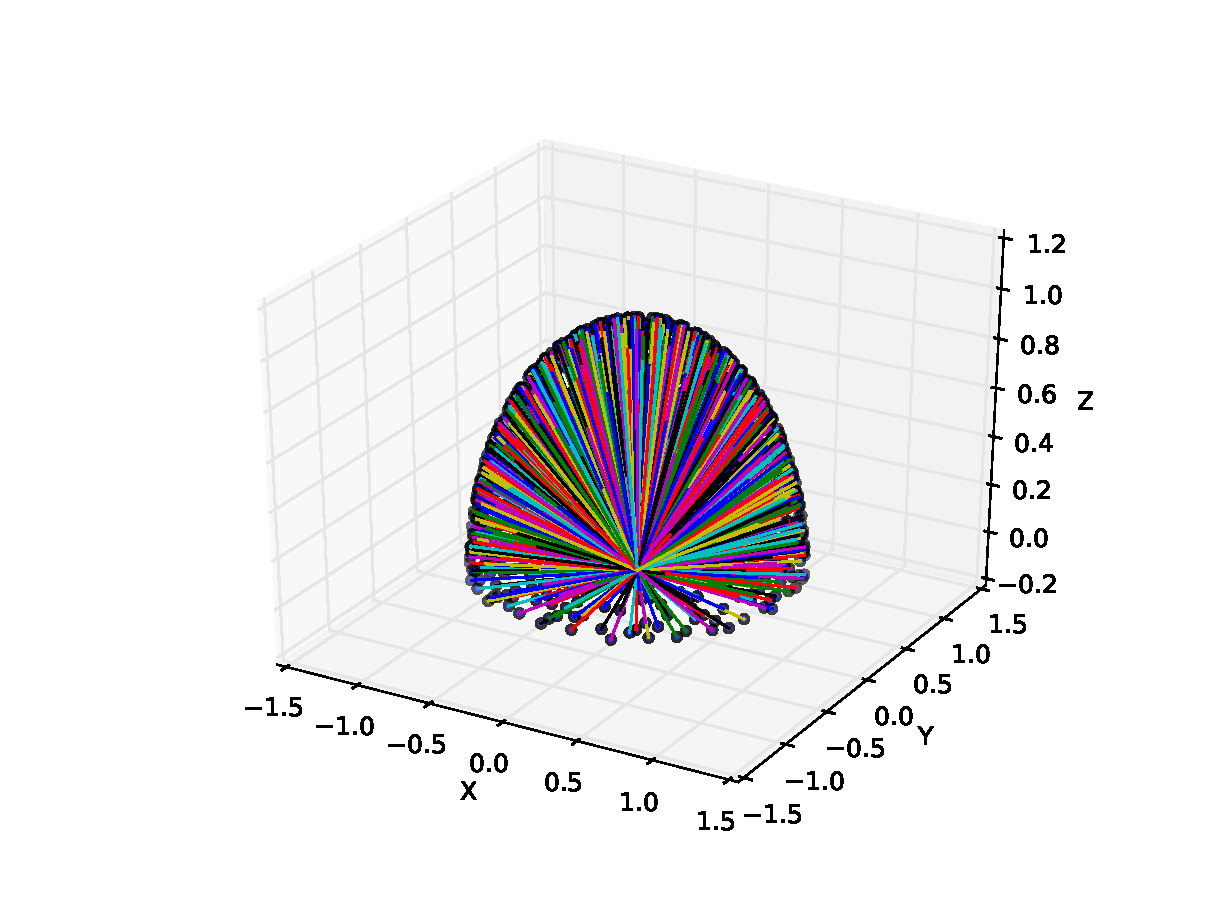
\includegraphics[height=0.7\textheight]{figs/freulon_algo_1000_bands.pdf}
\end{center}
\caption{1000 bands generated using the Freulon's algorithm}
\label{fig:freulon_algo_1000_bands}
\end{figure}
\end{frame}


\begin{frame}{Turning Bands: Generating the unidimensional simulations}
 
 The Turning Bands algorithm doesn't determine an algorithm to generate the independent stochastic process in each band. 
 Hence, in practice, for each model and band we generate independently the stochastic process using the appropriated 
 algorithm to the specific model. After the execution of all independent simulations in a direction $\theta_n$, 
 the results are combined to generate the final result in this direction. Emery \cite{emery2006tbsim} presents 15 algorithms
 to generate 15 different types of Covariance models.
 
\end{frame}

\begin{frame}
\frametitle{Conditioning the spectral simulations}
 In the previous slides, we presented some techniques to simulated the stochastic process associated with some types of covariances. Now,
 we will present the algorithm to generate the conditional simulations using Turning Bands (or other type of algorithm)
 in the simulation domain $D$. 
 In this algorithm, $CD$ stands the conditioning data-set.
 
\begin{block}{Conditional simulation of a Gaussian Random Function}
 \begin{enumerate}
  \item Calculate the kriged estimates $y^{*}(x)=\sum_c\lambda_c(x)y(c)$ for each $x \in D$.
  \item Simulate a gaussian random function (using Turning Bands or other type of simulation algorithm) with mean $0$ and covariance $C$
  in the domain $D$ and at the conditioning points. Let ($z(x), x \in D$) and ($z(c), c \in CD$) be the generated values.
  \item Calculate the kriged estimates $z^{*}(x) = \sum_c\lambda_c(x)z(c)$ for each $x \in D$.
  \item Return ($y^{*}(x) + z(x) - z^{*}(x), x \in D$).
 \end{enumerate}

\end{block}

\end{frame}


\begin{frame}{Turning Bands: some observations}
 \begin{itemize}
  \item The quality (convergence velocity) of the Turning Bands is directly related to the number of lines and to the algorithm
  used to generated the band directions.
  \item In the practice, using the Freulon's algorithm, a number of lines greater than 1000 is enough to generate good results \cite{emery2006tbsim}.
  \item When the number of lines is not appropriated, artifacts are generated.
  \item The Turning Bands is a \textit{share nothing} algorithm, so it's very easy to implement a highly efficient distributed version
  of this algorithm. The SGeMS has a very good implementation using openMP.
 \end{itemize}
\end{frame}


\begin{frame}{Turning Bands: the impact of the number of bands}
 
\begin{figure}
\begin{center}
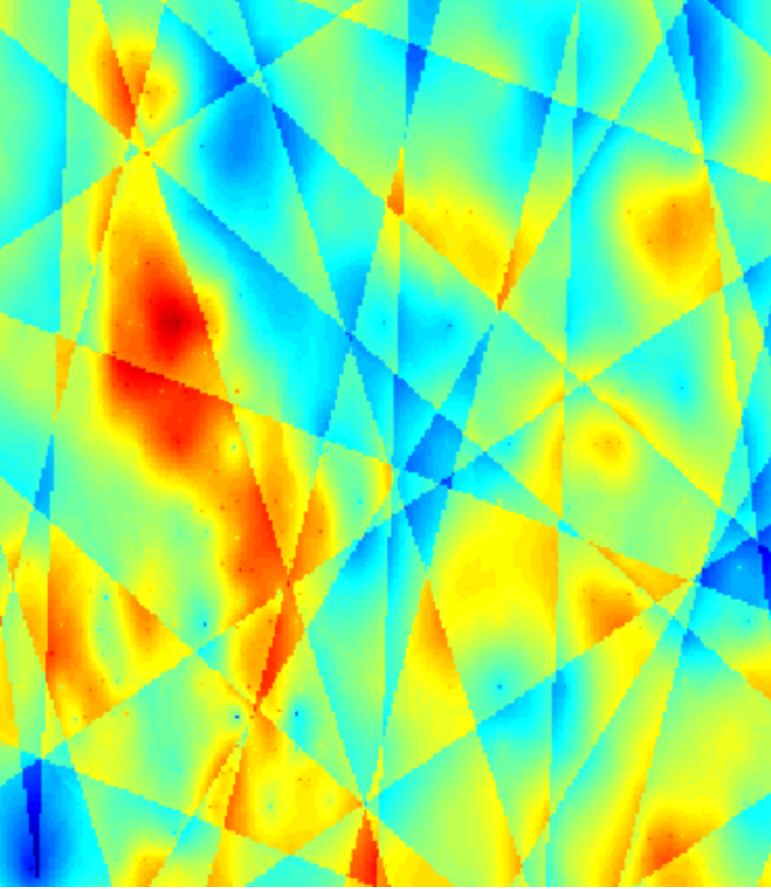
\includegraphics[width=0.5\textwidth]{figs/walker_lake_tb_n_10.pdf}
\end{center}
\caption{Conditional simulation of the Walker lake data-set with number of lines equals to 10.}
\label{fig:gaussian_unc_simulation}
\end{figure}
\end{frame}

\begin{frame}{Turning Bands: the impact of the number of bands}
\begin{figure}
\begin{center}
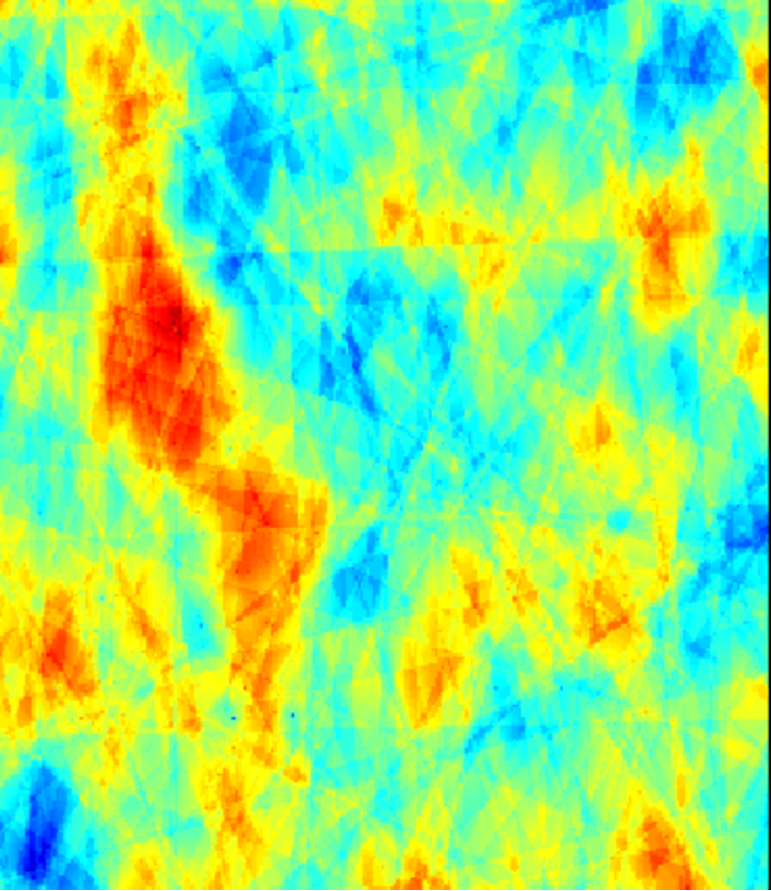
\includegraphics[width=0.5\textwidth]{figs/walker_lake_tb_n_100.pdf}
\end{center}
\caption{Conditional simulation of the Walker lake data-set with number of lines equals to 100.}
\label{fig:gaussian_unc_simulation}
\end{figure}
\end{frame}

\begin{frame}{Turning Bands: the impact of the number of bands}
\begin{figure}
\begin{center}
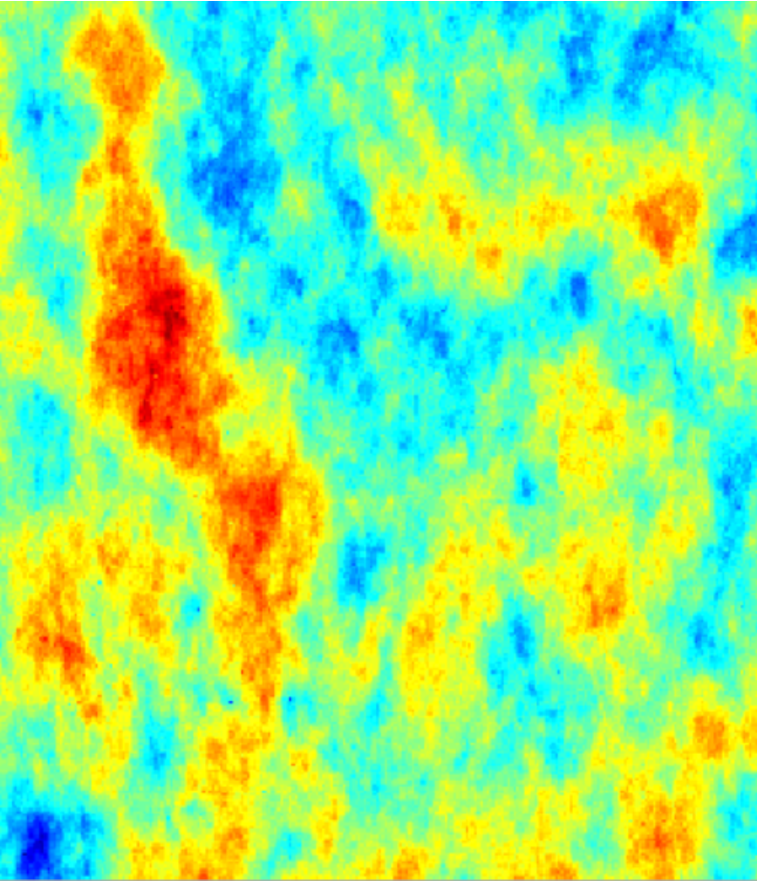
\includegraphics[width=0.5\textwidth]{figs/walker_lake_tb_n_1000.pdf}
\end{center}
\caption{Conditional simulation of the Walker lake data-set with number of lines equals to 1000.}
\label{fig:gaussian_unc_simulation}
\end{figure}
\end{frame}


\section{Final remarks}
\begin{frame}{Final remarks}
\begin{itemize}
	\item Fourier Integral Method and Turning Bands Simulation are very efficient simulation algorithm based in a problem transformation.
    \item The original simulation problem is transformed in M 1D independent simulations (in the band or in the phase).
    \item We can see the spectral simulation as a way to transform the geostatistical simulation in a embarrassingly problem. 
    \item We don't need to lead with random paths.
    \item Using covariance tables, we can reduce the modeling time generating the covariance model directly from data.
    \item Spectral allows the best usage of a modern computational infrastructure like GPUs, clusters, multi-core and modern APIs like GRPC, arrayfire, openmp, CUDA, and so on.
\end{itemize}
\end{frame}


\section{Final remarks}
\begin{frame}{Final remarks}
\begin{itemize}
	\item This is the thesis plan.
    \item In the next months, these will be implemented and the validity of results will be measured. 
\end{itemize}
\end{frame}





\section{Schedule}
\begin{frame}{Schedule}

\centering
\begin{table}
\centering
\begin{tabular}{l|r}
Period & Activity \\\hline
Jan. to Dec. 2017 & \textit{Ar2GeMS HPC} development \\
Jan. to Dec. 2017 & HPC spectral simulation development \\
Mar. to Dec. 2017 & Covariance table modeling development \\
Mar. to Dec. 2017 & Validations using real world scenarios \\
Mar. to Dec. 2017 & Validations using synthetic scenarios \\
Apr. 2017 to Dec. 2018 & Publish the results in journals  \\
Apr. 2018 to Dec. 2018 & Thesis writing 
\end{tabular}
\caption{\label{tab:widgets}Schedule.}
\end{table}


\end{frame}


\begin{frame}{Challenge Schedule}

\centering
\begin{table}
\centering
\begin{tabular}{l|r}
Period & Activity \\\hline
Jan. to Dec. 2017 & \textit{Ar2GeMS HPC} development \\
Jan. to Dec. 2017 & HPC spectral simulation development \\
Mar. to Jul. 2017 & Covariance table modeling development \\
Mar. to Jul. 2017 & Validations using real world scenarios \\
Mar. to Jul. 2017 & Validations using synthetic scenarios \\
Jul. 2017 to Dec. 2017 & Submit the results in journals  \\
Jul. 2017 to Dec. 2017 & Thesis writing 
\end{tabular}
\caption{\label{tab:widgets}Challenge Schedule.}
\end{table}


\end{frame}


\begin{frame}{Thank you!}
Obrigado!
\end{frame}


%%%%%%%%%%%%%%%%%%%%%%%%%%%%%%%%%%%%%%%%%%%%%%
\section{References}
\begin{frame}[allowframebreaks]{References}
\bibliography{bib/bib}
\end{frame}
%%%%%%%%%%%%%%%%%%%%%%%%%%%%%%%%%%%%%%%%%%%%%%


\end{document}
